\section{Tutorial A1}

\begin{problem}
    Determine whether each of the following systems of equations has a unique solution, infinitely many solutions, or no solutions. Find the solutions, where appropriate.

    \begin{enumerate}
        \item $\systeme{
            a + 2b - 3c = -5,
            -2a - 4b - 6c = 10,
            3a + 7b - 2c = -13
        }$
        \item $\systeme{
            x - y + 3z = 3,
            4x - 8y + 32z = 24,
            2x - 3y + 11z = 4
        }$
        \item $\systeme{
            x_1 + x_2 = 5,
            2x_1 + x_2 + x_3 = 13,
            4x_1 + 3x_2 + x_3 = 23
        }$
        \item $\systeme{
            1/p + 1/q + 1/r = 5,
            2/p - 3/q - 4/r = -11,
            3/p + 2/q - 1/r = -6
        }$
        \item $\systeme[\sin \cos \tan]{
            2\sin\a - \cos\b + 3\tan\g = 3,
            4\sin\a + 2\cos\b - 2\tan\g = 2,
            6\sin\a - 3\cos\b + \tan\g = 9
        }$, where $0 \leq \a \leq 2\pi$, $0 \leq \b \leq 2\pi$, and $0 \leq \g < \pi$.
    \end{enumerate}
\end{problem}
\begin{solution}
    \begin{ppart}
        Unique solution: $a = -9$, $b = 2$, $c = 0$.
    \end{ppart}
    \begin{ppart}
        No solution.
    \end{ppart}
    \begin{ppart}
        Infinitely many solutions: $x_1 = 8-t$, $x_2 = t-3$, $x_3 = t$.
    \end{ppart}
    \begin{ppart}
        Solving, we obtain \[\frac1p = 2, \quad \frac1q = -3, \quad \frac1r = 6.\] There is hence a unique solution: $p = \frac12$, $q = -\frac13$, $r = \frac16$.
    \end{ppart}
    \begin{ppart}
        Solving, we obtain \[\sin\a = 1, \quad \cos\b = -1, \quad \tan\g = 0.\] There is hence a unique solution: $\a = \frac\pi2$, $\b = \pi$, $\g = 0$.
    \end{ppart}
\end{solution}

\clearpage
\begin{problem}
    The following figure shows the circular cross-section of a uniform log floating in a canal.

    \begin{center}
        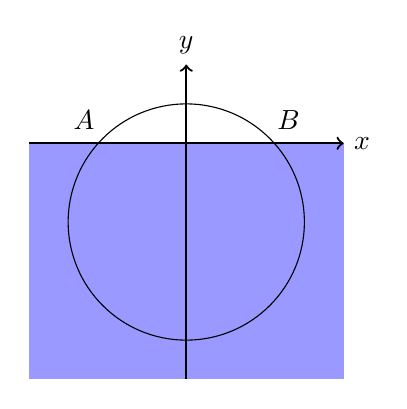
\begin{tikzpicture}
            \fill[blue!40!white] (0,0) rectangle (4,3);
            \draw (2,2) circle (1.5cm);
            \draw[thick,->] (0,3) -- (4,3) node[anchor=west] {$x$};
            \draw[thick,->] (2,0) -- (2,4) node[anchor=south] {$y$};
            \node[align=left] at (0.7, 3.3) {$A$};
            \node[align=left] at (3.3, 3.3) {$B$};
        \end{tikzpicture}
    \end{center}
    
    With respect to the axes shown, the circular outline of the log can be modelled by the equation \[x^2 + y^2 + ax + by + c = 0.\]

    $A$ and $B$ are points on the outline that lie on the water surface. Given that the highest point of the log is 1-cm above the water surface when $AB$ is 40 cm apart horizontally, determine the values of $a$, $b$ and $c$ by forming a system of linear equations.
\end{problem}
\begin{solution}
    Since $AB = 40$, we have $A(-20, 0)$ and $B(20, 0)$. We also know $(0, 10)$ lies on the circle. Substituting these points into the given equation, we have the following system of equations: \[\systeme{-20a + c = -400, 20a + c = -400, 10b + c = -100}\] Solving, we obtain $a = 0$, $b = 30$, $c = -400$.
\end{solution}

\begin{problem}
    Find the exact solution set of the following inequalities.

    \begin{enumerate}
        \item $x^2 - 2 \geq 0$
        \item $4x^2 - 12x + 10 > 0$
        \item $x^2 + 4x + 13 < 0$
        \item $x^3 < 6x - x^2$
        \item $x^2(x-1)(x+3) \geq 0$
    \end{enumerate}
\end{problem}
\begin{solution}
    \begin{ppart}
        Note that $x^2 - 2 \geq 0 \implies x \leq -\sqrt{2} \lor x \geq \sqrt{2}$. The solution set is thus $\bc{x \in \RR \colon x \leq -\sqrt2 \lor x \geq \sqrt2}$.
    \end{ppart}
    \begin{ppart}
        Completing the square, we see that $4x^2 - 12x + 10 > 0 \implies (x-\frac32)^2 + \frac{19}4 > 0$. Since $(x-\frac32)^2 \geq 0$, all $x \in \RR$ satisfy the inequality, whence the solution set is $\RR$.
    \end{ppart}
    \begin{ppart}
        Completing the square, we have $x^2 + 4x + 13 < 0 \implies (x+2)^2 + 9 < 0$. Since $\bp{x+2}^2 \geq 0$, there is no solution to the inequality, whence the solution set is $\varnothing$.
    \end{ppart}
    \begin{ppart}
        Note that $x^3 < 6x - x^2 \implies x(x+3)(x-2) < 0$.
        \begin{center}
            \begin{tikzpicture}
                \draw[-latex] (-4,0) -- (3,0) node[right]{$x$};
                \foreach \x in  {-3, 0, 2}
                \draw[shift={(\x,0)}] (0pt,3pt) -- (0pt,-3pt);
                \foreach \x in {-3, 0, 2}
                \draw[shift={(\x,-3pt)}] node[below] 
                {$\x$};
                \draw[very thick, -o, color=red] (-4, 0) -- (-2.88, 0);
                \draw[very thick, o-o, color=red] (-0.12, 0) -- (2.12, 0);
                \node[anchor=south, align=center] at (-3.5, 0) {$-$};
                \node[anchor=south, align=center] at (-1.5, 0) {$+$};
                \node[anchor=south, align=center] at (1, 0) {$-$};
                \node[anchor=south, align=center] at (2.5, 0) {$+$};
            \end{tikzpicture}
        \end{center}
        The solution set is thus $\bc{x \in \RR \colon x < -3 \lor 0 < x < 2}$.
    \end{ppart}
    \begin{ppart}
        \begin{center}
            \begin{tikzpicture}
                \draw[-latex] (-4,0) -- (2,0) node[right]{$x$};
                \foreach \x in  {-3, 0, 1} \draw[shift={(\x,0)}] (0pt,3pt) -- (0pt,-3pt);
                \foreach \x in {-3, 0, 1} \draw[shift={(\x,-3pt)}] node[below] {$\x$};

                \draw[very thick, -*, color=red] (-4, 0) -- (-2.88, 0);
                \draw[very thick, *-, color=red] (0.88, 0) -- (1.9, 0);
                \path [draw=red, fill=red] (0,0) circle (3pt);

                \node[anchor=south, align=center] at (-3.5, 0) {$+$};
                \node[anchor=south, align=center] at (-1.5, 0) {$-$};
                \node[anchor=south, align=center] at (0.5, 0) {$-$};
                \node[anchor=south, align=center] at (1.5, 0) {$+$};
            \end{tikzpicture}
        \end{center}
        The solution set is thus $\bc{x \in \RR \colon x \leq -3 \lor x = 0 \lor x \geq 1}$.
    \end{ppart}
\end{solution}

\begin{problem}
    Find the exact solution set of the following inequalities.

    \begin{enumerate}
        \item $\abs{3x+5} < 4$
        \item $\abs{x-2} < 2x$
    \end{enumerate}
\end{problem}
\begin{solution}
    \begin{ppart}
        If $3x + 5 < 4$, then $x < -\frac13$. If $-(3x+5) < 4$, then $x > -3$. Combining both inequalities, we have $-3 < x < -\frac13$. Thus, the solution set is $\bc{x \in \RR \colon -3 < x< -\frac13}$.
    \end{ppart}
    \begin{ppart}
        If $x - 2 < 2x$, then $x > -2$. If $-(x-2) < 2x$, then $x > \frac23$. Combining both inequalities, we have $x > \frac23$. Thus, the solution set is $\bc{x \in \RR \colon x > \frac23}$.
    \end{ppart}
\end{solution}

\begin{problem}
    It is given that $p(x) = x^4 + ax^3 + bx^2 + cx + d$, where $a$, $b$, $c$ and $d$ are constants. Given that the curve with equation $y = p(x)$ is symmetrical about the $y$-axis, and that it passes through the points with coordinates $(1, 2)$ and $(2, 11)$, find the values of $a$, $b$, $c$ and $d$.
\end{problem}
\begin{solution}
    We know that $(1, 2)$ and $(2, 11)$ lie on the curve. Since $y = p(x)$ is symmetrical about the $y$-axis, we have that $(-1, 2)$ and $(-2, 11)$ also lie on the curve. Substituting these points into $y = p(x)$, we obtain the following system of equations:
    \[
        \systeme{
            a+b+c+d = 1,
            a-b+c-d = -1,
            8a+4b+2c+d = -5,
            8a-4b+2c-d = 5
        }
    \]
    Solving, we obtain $a = 0$, $b = -2$, $c = 0$, $d=3$.
\end{solution}

\begin{problem}
    Mr Mok invested \$50,000 in three funds A, B and C. Each fund has a different risk level and offers a different rate of return.

    In 2016, the rates of return for funds A, B and C were 6\%, 8\%, and 10\% respectively and Mr Mok attained a total return of \$3,700. He invested twice as much money in Fund A as in Fund C. How much did he invest in each of the funds in 2016?
\end{problem}
\begin{solution}
    Let $a$, $b$ and $c$ be the amount of money Mr Mok invested in Funds A, B and C respectively, in dollars. We thus have the following system of equations.
    \[
        \systeme{
            a+b+c = 50000,
            \frac{6}{100}a + \frac{8}{100}b + \frac{10}{100}c = 3700,
            a = 2c
        }
    \]
    Solving, we have $a = 30000$, $b = 5000$ and $c = 15000$. Thus, Mr Mok invested \$30,000, \$5,000 and \$15,000 in Funds A, B and C respectively.
\end{solution}

\begin{problem}
    Solve the following inequalities with exact answers.

    \begin{enumerate}
        \item $2x-1 \geq \frac6x$
        \item $x-\frac1x < 1$
        \item $-1 < \frac{2x+3}{x-1} < 1$
    \end{enumerate}
\end{problem}
\begin{solution}
    \begin{ppart}
        Note that $x \neq 0$. \[2x-1 \geq \frac6x \implies x^2(2x-1) \geq 6x \implies x\bp{2x^2-x-6} \geq 0 \implies x(2x+3)(x-2) \geq 0.\]

        \begin{center}
            \begin{tikzpicture}
                \draw[-latex] (-2.5,0) -- (3,0) node[right]{$x$};
                \foreach \x in  {-1.5, 0, 2}
                \draw[shift={(\x,0)}] (0pt,3pt) -- (0pt,-3pt);
                \foreach \x in {-1.5, 0, 2}
                \draw[shift={(\x,-3pt)}] node[below] 
                {$\x$};

                \draw[very thick, *-o, color=red] (-1.6, 0) -- (0.12, 0);
                \draw[very thick, *-, color=red] (1.9, 0) -- (2.9, 0);

                \node[anchor=south, align=center] at (-2, 0) {$-$};
                \node[anchor=south, align=center] at (-0.75, 0) {$+$};
                \node[anchor=south, align=center] at (1, 0) {$-$};
                \node[anchor=south, align=center] at (2.5, 0) {$+$};
            \end{tikzpicture}
        \end{center}
        Thus, $-\frac32 \leq x < 0 \lor x \geq 2$.
    \end{ppart}
    \begin{ppart}
        Note that $x \neq 0$. \[x - \frac1x < 1 \implies x^3 - x < x^2 \implies x\bp{x^2 - x - 1} < 0 \implies x(x-\vf)(x-\ol{\vf}) < 0.\]

        \begin{center}
            \begin{tikzpicture}
                \draw[-latex] (-1.618,0) -- (2.618,0) node[right]{$x$};
                \foreach \x in  {-0.618, 0, 1.618}
                \draw[shift={(\x,0)}] (0pt,3pt) -- (0pt,-3pt);

                \draw[shift={(-0.618,-3pt)}] node[below] 
                {$\ol{\vf}$};
                \draw[shift={(0,-3pt)}] node[below] 
                {0};
                \draw[shift={(1.618,-3pt)}] node[below] 
                {$\vf$};

                \draw[very thick, -*, color=red] (-1.618, 0) -- (-0.518, 0);
                \draw[very thick, o-*, color=red] (-0.12, 0) -- (1.718, 0);

                \node[anchor=south, align=center] at (-1.118, 0) {$-$};
                \node[anchor=south, align=center] at (-0.309, 0) {$+$};
                \node[anchor=south, align=center] at (0.809, 0) {$-$};
                \node[anchor=south, align=center] at (2.118, 0) {$+$};
            \end{tikzpicture}
        \end{center}
        Thus, $x \leq \bar{\vf} \lor 0 < x \leq \vf$.
    \end{ppart}
    \begin{ppart}
        \[-1 < \frac{2x+3}{x-1} < 1 \implies -3 < \frac5{x-1} < -1 \implies -\frac35 < \frac1{x-1} < -\frac15 \implies -4 < x < -\frac23.\]
    \end{ppart}
\end{solution}

\begin{problem}
    Without using a calculator, solve the inequality $\frac{x^2+x+1}{x^2+x-2} < 0$.
\end{problem}
\begin{solution}
    Observe that $x^2 + x + 1 = \bp{x + \frac12}^2 + \frac34 > 0$. The inequality thus reduces to $\frac1{x^2+x-2} < 0$. \[\frac1{x^2+x-2} < 0 \implies x^2 + x - 2 < 0 \implies (x-1)(x+2) < 0.\]

    \begin{center}
        \begin{tikzpicture}
            \draw[-latex] (-3,0) -- (2,0) node[right]{$x$};
            \foreach \x in  {-2, 1}
            \draw[shift={(\x,0)}] (0pt,3pt) -- (0pt,-3pt);

            \foreach \x in  {-2, 1}
            \draw[shift={(\x,-3pt)}] node[below] 
            {$\x$};

            \draw[very thick, o-o, color=red] (-2.12, 0) -- (1.12, 0);

            \node[anchor=south, align=center] at (-2.5, 0) {$+$};
            \node[anchor=south, align=center] at (-0.5, 0) {$-$};
            \node[anchor=south, align=center] at (1.5, 0) {$+$};
        \end{tikzpicture}
    \end{center}
    Hence, $-2 < x < 1$.
\end{solution}

\clearpage
\begin{problem}
    Solve the following inequalities using a graphical method.

    \begin{enumerate}
        \item $\abs{3x+1} < (4x+3)^2$
        \item $\abs{3x+1} \geq \abs{2x+7}$
        \item $\abs{x-2} \geq x + \abs{x}$
        \item $5x^2 + 4x - 3 > \ln{x+1}$
    \end{enumerate}
\end{problem}
\begin{solution}
    \begin{ppart}
        \begin{center}
            \begin{tikzpicture}[trim axis left, trim axis right]
                \begin{axis}[
                    domain = -2.5:0.5,
                    samples = 50,
                    axis y line=middle,
                    axis x line=middle,
                    xlabel = {$x$},
                    ylabel = {$y$},
                    xtick = {-0.75},
                    xticklabels = {$-\frac34$},
                    ytick = {1, 9},
                    ymax=10,
                    legend cell align={left},
                    legend pos=outer north east,
                    after end axis/.code={\path (axis cs:0,0) node [anchor=north] {$O$};}]
                    
                    \addplot[plotRed, name path=f1] {abs(3*x+1)};

                    \addlegendentry{$y=\abs{3x+1}$};

                    \addplot[plotBlue, name path=f2] {(4*x+3)^2};

                    \addlegendentry{$y=(4x+3)^2$};

                    \fill [name intersections={of=f1 and f2,by={E1,E2}}] (E1) circle[radius=2.5pt] node[anchor=south east, fill=white, opacity = 0.6, text opacity=1] {$(-1.14, 2.42)$};
                    
                    \fill (E2) circle[radius=2.5pt] node[anchor=south east, fill=white, opacity = 0.6, text opacity=1] {$(-0.549, 0.647)$};
                \end{axis}
            \end{tikzpicture}
        \end{center}
        Thus, $x < -1.14 \lor x > -0.549$.
    \end{ppart}
    \begin{ppart}
        \begin{center}
            \begin{tikzpicture}[trim axis left, trim axis right]
                \begin{axis}[
                    domain = -6:8,
                    samples = 50,
                    axis y line=middle,
                    axis x line=middle,
                    xlabel = {$x$},
                    ylabel = {$y$},
                    xtick = {-3.5, -0.333},
                    xticklabels = {$-\frac72$, $-\frac13$},
                    ytick = {1, 7},
                    ymax=20,
                    legend cell align={left},
                    legend pos=outer north east,
                    after end axis/.code={
                        \path (axis cs:0,0) 
                            node [anchor=north west] {$O$};
                        }
                    ]
                    \addplot[plotRed, name path=f1] {abs(3*x+1)};

                    \addlegendentry{$y=\abs{3x+1}$};

                    \addplot[plotBlue, name path=f2] {abs(2*x + 7)};

                    \addlegendentry{$y=\abs{2x+7}$};

                    \fill [name intersections={of=f1 and f2,by={E1,E2}}] (E1) circle[radius=2.5pt] node[anchor=east] {$(-1.6, 3.8)$};
                    
                    \fill (E2) circle[radius=2.5pt] node[anchor=east] {$(6, 19)$};
                \end{axis}
            \end{tikzpicture}
        \end{center}
        Thus, $x \leq -1.6 \lor x \geq 6$.
    \end{ppart}

    \clearpage
    \begin{ppart}
        \begin{center}
            \begin{tikzpicture}[trim axis left, trim axis right]
                \begin{axis}[
                    domain = -0.5:2.5,
                    samples = 50,
                    axis y line=middle,
                    axis x line=middle,
                    xlabel = {$x$},
                    ylabel = {$y$},
                    xtick = {2},
                    ytick = {2},
                    ymax=2.5,
                    legend cell align={left},
                    legend pos=outer north east,
                    after end axis/.code={
                        \path (axis cs:0,0) 
                            node [anchor=north] {$O$};
                        }
                    ]
                    \addplot[plotRed, name path=f1] {abs(x-2)};

                    \addlegendentry{$y=\abs{x-2}$};

                    \addplot[plotBlue, name path=f2] {x + abs(x)};

                    \addlegendentry{$y=x+\abs{x}$};

                    \fill [name intersections={of=f1 and f2,by={E1}}] (E1) circle[radius=2.5pt] node[anchor=west] {$(0.667, 1.33)$};
                \end{axis}
            \end{tikzpicture}
        \end{center}
        Thus, $x \leq 0.667$.
    \end{ppart}
    \begin{ppart}
        \begin{center}
            \begin{tikzpicture}[trim axis left, trim axis right]
                \begin{axis}[
                    domain = -2.3:3,
                    samples = 200,
                    axis y line=middle,
                    axis x line=middle,
                    xlabel = {$x$},
                    ylabel = {$y$},
                    ymax=3,
                    xtick = {-1.27, 0.472},
                    ytick = {-3},
                    legend cell align={left},
                    legend pos=outer north east,
                    after end axis/.code={
                        \path (axis cs:0,0) 
                            node [anchor=south east] {$O$};
                        }
                    ]
                    \addplot[plotRed, name path=f1] {5*x^2 + 4*x -3};

                    \addlegendentry{$y=5x^2+4x-3$};

                    \addplot[plotBlue, name path=f2] {ln(x+1)};

                    \addlegendentry{$y=\ln{x+1}$};

                    \fill [name intersections={of=f1 and f2,by={E1, E2}}] (E1) circle[radius=2.5pt] node[anchor=south west, fill=white, opacity = 0.6, text opacity=1] {$(-0.916, -2.47)$};

                    \fill (E2) circle[radius=2.5pt] node[anchor=south west, fill=white, opacity = 0.6, text opacity=1] {$(0.518, 0.418)$};

                    \addplot[mark=none, black, thick, dotted] coordinates {(-1, 5) (-1,-4)};

                    \node[anchor=north east, fill=white, opacity = 0.6, text opacity=1] at (axis cs:-1, 3) {$x = -1$};

                    \addplot[mark=none, white!100] {-4};
                \end{axis}
            \end{tikzpicture}
        \end{center}
        Thus, $-1 < x < -0.916 \lor x > 0.518$.
    \end{ppart}
\end{solution}

\begin{problem}
    Sketch the graphs of $y = \abs{x-20}$ and $y=\frac1x$ on the same diagram. Hence or otherwise, solve the inequality $\abs{x-20} < \frac1x$, leaving your answers correct to 2 decimal places.
\end{problem}
\begin{solution}
    \begin{center}
        \begin{tikzpicture}[trim axis left, trim axis right, scale=0.95]
            \begin{axis}[
                domain = -5:36,
                samples = 83,
                axis y line=middle,
                axis x line=middle,
                xlabel = {$x$},
                ylabel = {$y$},
                ymax=25,
                ymin=-20,
                legend cell align={left},
                legend pos=outer north east,
                xtick={20},
                ytick = {20},
                after end axis/.code={
                    \path (axis cs:0,0) 
                        node [anchor=north east] {$O$};
                    }
                ]
                \addplot[plotRed, name path=f1] {abs(x-20)};

                \addlegendentry{$y = \abs{x-20}$};

                \addplot[plotBlue, name path=f2, unbounded coords=jump] {50 /x};

                \addlegendentry{$y=x^{-1}$};

                \fill [name intersections={of=f1 and f2,by={E1, E2, E3}}] (E1) circle[radius=2.5pt] node[anchor=north west, fill=white, opacity = 0.6, text opacity=1] {$(0.05, 19.95)$};

                \fill (E2) circle[radius=2.5pt] node[anchor=south east, fill=white, opacity = 0.6, text opacity=1] {$(19.05, 0.05)$};

                \fill (E3) circle[radius=2.5pt] node[anchor=south west, fill=white, opacity = 0.6, text opacity=1] {$(20.05, 0.05)$};
            \end{axis}
        \end{tikzpicture}
    \end{center}
    Thus, $0 < x < 0.05 \lor 19.95 < x < 20.05$.
\end{solution}

\begin{problem}
    Solve the inequality $\frac{x-9}{x^2-9} \leq 1$. Hence, solve the inequalities

    \begin{enumerate}
        \item $\frac{\abs{x}-9}{x^2-9} \leq 1$
        \item $\frac{x+9}{x^2-9} \geq -1$
    \end{enumerate}
\end{problem}
\begin{solution}
    Note that $x^2 - 9 \neq 0 \implies x \neq \pm 3$.
    \[\frac{x-9}{x^2-9} \leq 1 \implies (x-9)\bp{x^2-9} \leq \bp{x^2 - 9}^2.\] Expanding and factoring, we get \[x^4 - x^3 - 9x^2 + 9x = x(x+3)(x-1)(x-3) \geq 0.\]

    \begin{center}
        \begin{tikzpicture}
            \draw[-latex] (-4,0) -- (4,0) node[right]{$x$};
            \foreach \x in  {-3, 0, 1, 3}
            \draw[shift={(\x,0)}] (0pt,3pt) -- (0pt,-3pt);
            \foreach \x in  {-3, 0, 1, 3}
            \draw[shift={(\x,-3pt)}] node[below] 
            {$\x$};

            \draw[very thick, -o, color=red] (-4, 0) -- (-2.88, 0);
            \draw[very thick, *-*, color=red] (-0.12, 0) -- (1.12, 0);
            \draw[very thick, o-, color=red] (2.88, 0) -- (3.9, 0);


            \node[anchor=south, align=center] at (-3.5, 0) {$+$};
            \node[anchor=south, align=center] at (-1.5, 0) {$-$};
            \node[anchor=south, align=center] at (0.5, 0) {$+$};
            \node[anchor=south, align=center] at (3.5, 0) {$-$};
        \end{tikzpicture}
    \end{center}
    Thus, $x < -3 \lor 0 \leq x \leq 1 \lor x > 3$.

    \begin{ppart}
        Consider the substitution $x \mapsto \abs{x}$. Then \[\abs{x} < -3 \lor 0 \leq \abs{x} \leq 1 \lor \abs{x} > 3.\] This immediately gives us $x < -3 \lor -1 \leq x \leq 1 \lor x > 3$.
    \end{ppart}
    \begin{ppart}
        Consider the substitution $x \mapsto -x$. Then \[-x < -3 \lor 0 \leq -x \leq 1 \lor -x > 3.\] This immediately gives us $x < -3 \lor -1 \leq x \leq 0 \lor x > 3$.
    \end{ppart}
\end{solution}

\begin{problem}
    Solve the inequality $\frac{x-5}{1-x} \geq 1$. Hence, solve $0 < \frac{1-\ln x}{\ln x -5} \leq 1$.
\end{problem}
\begin{solution}
    Note that $x \neq 1$. \[\frac{x-5}{1-x} \geq 1 \implies  (x-5)(1-x) \geq \bp{1-x}^2 \implies 2x^2-8x+6 \leq 0 \implies 2(x-1)(x-3) \leq 0.\]

    \begin{center}
        \begin{tikzpicture}
            \draw[-latex] (0,0) -- (4,0) node[right]{$x$};
            \foreach \x in  {1, 3}
            \draw[shift={(\x,0)}] (0pt,3pt) -- (0pt,-3pt);
            \foreach \x in  {1, 3}
            \draw[shift={(\x,-3pt)}] node[below] 
            {$\x$};

            \draw[very thick, o-*, color=red] (0.88, 0) -- (3.12, 0);


            \node[anchor=south, align=center] at (0.5, 0) {$+$};
            \node[anchor=south, align=center] at (2, 0) {$-$};
            \node[anchor=south, align=center] at (3.5, 0) {$+$};
        \end{tikzpicture}
    \end{center}
    Thus, $1 < x \leq 3$.

    Consider the substitution $x \mapsto \ln x$. Taking reciprocals, we have our desired inequality $0 < \frac{1-\ln x}{\ln x -5} \leq 1$. Hence, \[1 < \ln x \leq 3 \implies e < x \leq e^3.\]
\end{solution}

\begin{problem}
    A small rocket is launched from a height of 72 m from the ground. The height of the rocket in metres, $h$, is represented by the equation $h = -16t^2 + 64t+72$, where $t$ is the time in seconds after the launch.

    \begin{enumerate}
        \item Sketch the graph of $h$ against $t$.
        \item Determine the number of seconds that the rocket will remain at or above 100 m from the ground.
    \end{enumerate}
\end{problem}
\begin{solution}
    \begin{ppart}
        \begin{center}
            \begin{tikzpicture}[trim axis left, trim axis right]
                \begin{axis}[
                    domain = 0:5.5,
                    samples = 101,
                    axis y line=middle,
                    axis x line=middle,
                    xlabel = {$t$},
                    ylabel = {$h$},
                    xtick={4.92},
                    xticklabels={4.92},
                    ytick={136},
                    yticklabels={136},
                    ymax=165,
                    legend cell align={left},
                    legend pos=outer north east,
                    after end axis/.code={
                        \path (axis cs:0,0) 
                            node [anchor=north east] {$O$};
                        }
                    ]

                    \fill (2, 136) circle (3pt) node[anchor=south west] {$(2, 136)$};

                    \addplot[plotRed, domain=0:4.92] {-16*x^2 + 64*x + 72)};

                    \addlegendentry{$h = -16t^2 + 64t+72$};

                    \addplot[white!0]{165};
                \end{axis}
            \end{tikzpicture}
        \end{center}
    \end{ppart}
    \begin{ppart}
        Note that $-16t^2 + 64t+72 \geq 100 \implies -4(2t-1)(2t-7) \geq 0$.

        \begin{center}
            \begin{tikzpicture}
                \draw[-latex] (-0.5,0) -- (4.5,0) node[right]{$x$};
                \foreach \x in  {0.5, 3.5}
                \draw[shift={(\x,0)}] (0pt,3pt) -- (0pt,-3pt);
                \foreach \x in  {0.5, 3.5}
                \draw[shift={(\x,-3pt)}] node[below] 
                {$\x$};

                \draw[very thick, *-*, color=red] (0.38, 0) -- (3.65, 0);
    
                \node[anchor=south, align=center] at (0, 0) {$-$};
                \node[anchor=south, align=center] at (2,0) {$+$};
                \node[anchor=south, align=center] at (4, 0) {$-$};
            \end{tikzpicture}
        \end{center}
        Thus, the rocket will remain at or above 100 m from the ground for 3 seconds.
    \end{ppart}
\end{solution}

\begin{problem}
    Xinxin, a new graduate, starts work at a company with an initial monthly pay of \$2,000. For every subsequent quarter that she works, she will get a pay increase of 5\%, leading to a new monthly pay of $2000(1.05)^{n-1}$ dollars in the $n$th quarter, where $n$ is a positive integer. She also gives a regular donation of \$$300n$ in the $n$th quarter that she works. However, she will stop the donation when her monthly pay falls below the donation amount. At which quarter will this first happen?
\end{problem}
\begin{solution}
    Consider the curves $y = 2000(1.05)^{x-1}$ and $y=300x$.

    \begin{center}
        \begin{tikzpicture}[trim axis left, trim axis right]
            \begin{axis}[
                domain = 0:13,
                samples = 81,
                axis y line=middle,
                axis x line=middle,
                xlabel = {$x$},
                ylabel = {$y$},
                legend cell align={left},
                legend pos=outer north east,
                xticklabels={20},
                xtick={20},
                ymajorticks=false,
                after end axis/.code={
                    \path (axis cs:0,0) 
                        node [anchor=north east] {$O$};
                    }
                ]
                \addplot[plotRed, name path=f1] {2000 * (1.05)^(x-1)};

                \addlegendentry{$y = 2000(1.05)^{x-1}$};

                \addplot[plotBlue, name path=f2] {300*x};

                \addlegendentry{$y=300x$};

                \fill [name intersections={of=f1 and f2,by={E1}}] (E1) circle[radius=2.5pt] node[anchor=south east] {$(10.7, 3210)$};
            \end{axis}
        \end{tikzpicture}
    \end{center}
    Hence, Xinxin will stop donating in the 11th quarter.
\end{solution}